\documentclass[12pt,a4paper,utf8]{ctexart}
\usepackage{graphicx}
\usepackage{amsmath}
\usepackage{amssymb}
\usepackage{subfig}
\usepackage{cite}
\usepackage[ntheorem]{empheq}
\usepackage{enumitem}
\usepackage{fullpage}
\usepackage{cleveref}
\usepackage{cellspace}
\usepackage{listings}
\usepackage{color}
\usepackage{float}
\definecolor{gray}{rgb}{0.5,0.5,0.5}
\definecolor{dkgreen}{rgb}{.068,.578,.068}
\definecolor{dkpurple}{rgb}{.320,.064,.680}

% set Matlab styles
\lstset{
	language=Matlab,
	keywords={break,case,catch,continue,else,elseif,end,for,function,
		global,if,otherwise,persistent,return,switch,try,while},
	basicstyle=\ttfamily,
	keywordstyle=\color{blue}\bfseries,
	commentstyle=\color{dkgreen},
	stringstyle=\color{dkpurple},
	backgroundcolor=\color{white},
	tabsize=4,
	showspaces=false,
	showstringspaces=false
}

\begin{document}
	\CJKfamily{zhkai}	
	
	
	\begin{center}
		\textbf{作业三}\\
		\textbf{姓名 ~~~~~~~~~~~~~ 学号 ~~~~~~~~~~~~~~ 日期}\\
	\end{center}
	
	\begin{center}
		\fbox{
			\begin{minipage}{40em}
				\vspace{5cm}
				\hspace{18cm}
		\end{minipage}}
	\end{center}
	\vspace{1cm}
	
	\begin{enumerate}
		\item[第一题] \textbf{本题考虑使用Richardson外推技术提高向前差商求给定函数导数的精度。} 
		\item[(a)](5分)使用向前差分计算$f(x) = \sin(x)$在$x = 1.2$处的导数并使用\textbf{loglog}图展示其精度随离散区间大小$h$的变化。$h$取$10^0, 10^{−1},10^{−2},10^{−3},...,10^{−15}$。\\
		\begin{figure}[H]  
			\centering
			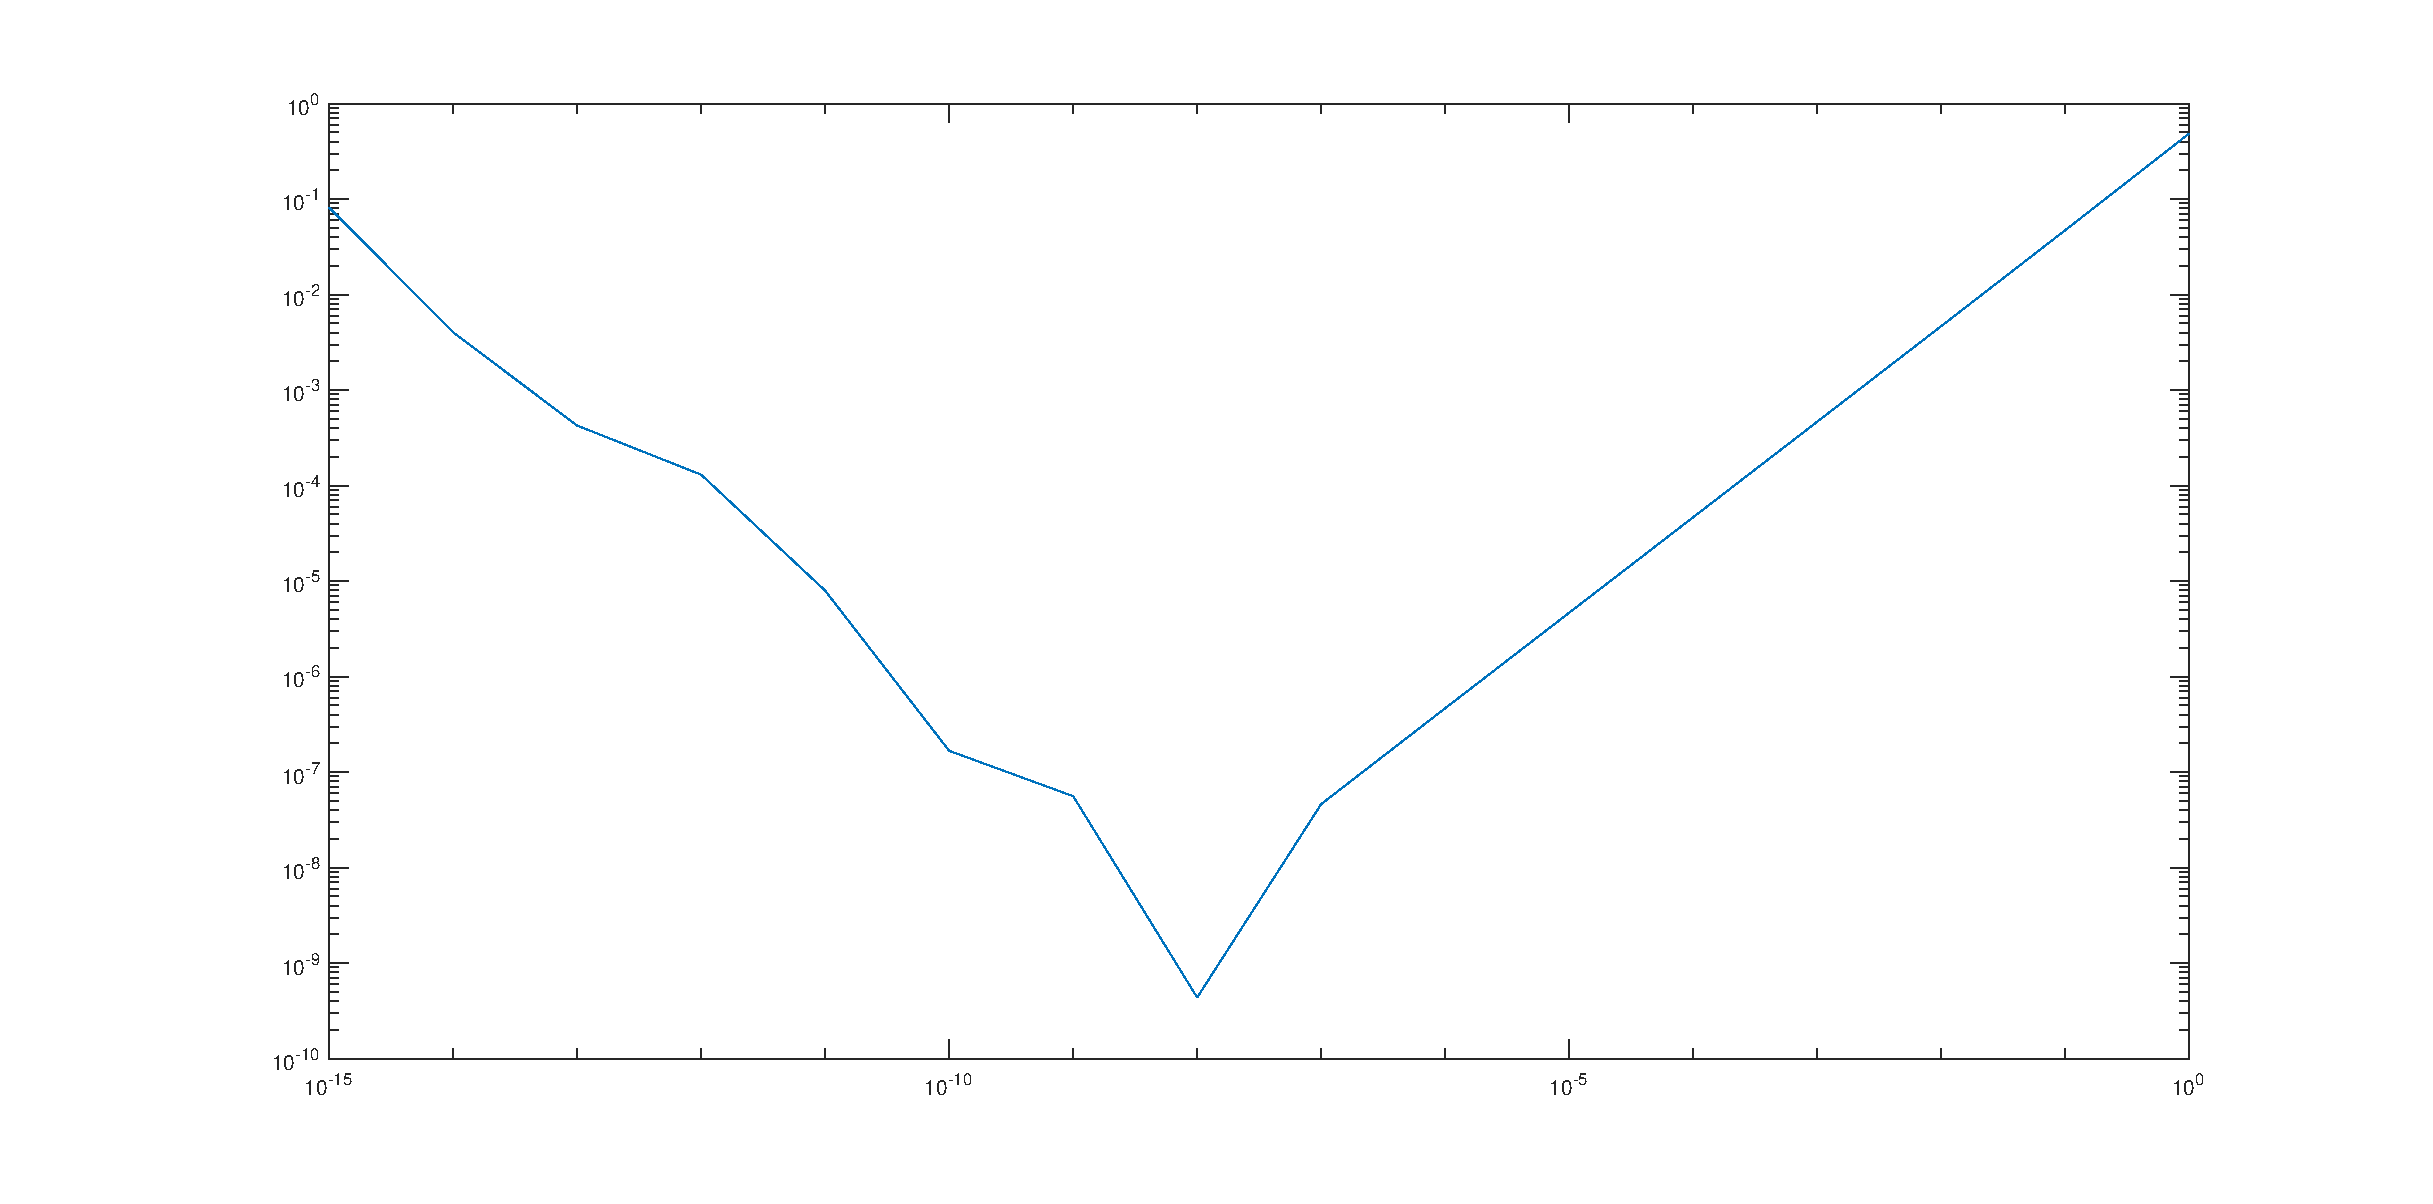
\includegraphics[width=\textwidth]{loglog1}
			\caption{精度随离散区间的变化}  
			\label{1}  
		\end{figure}
		\item[(b)](10分)推导出使用\textbf{Richardson}外推技术的向前差商的计算公式并用伪代码给出算法。\\
		答:\\
		由泰勒展开知$$
		f(x_{0}+h)=f(x_{0})+hf^{'}(x_{0})+\frac{h^{2}}{2!}f^{''}(x_{0})+O(h^{3})$$
		因此$$
		\frac{f(x_{0}+h)-f(x_{0})}{h}=f^{'}(x_{0})+\frac{h}{2!}f^{''}(x_{0})+O(h^2)
		$$记$$N_{1}(h)=\frac{f(x_{0}+h)-f(x_{0})}{h}$$
		$$f^{'}(x_{0})=N_{1}(h)-\frac{h}{2!}f^{''}(x_{0})+O(h^{2})$$
		$$f^{'}(x_{0})=N_{1}(\frac{h}{2})-\frac{h}{4}f^{''}(x_{0})+O(h^{2})$$
		两式联立得到:
		$$f^{'}(x_{0})=2N_{1}(\frac{h}{2})-N_{1}(h)+O(h^{2})$$
		记$$N_{2}(h)=2N_{1}(\frac{h}{2})-N_{1}(h)$$
		则$$f^{'}(x_{0})=N_{2}(h)+\frac{h^{2}}{12}f^{'''}(x_{0})+O(h^{4})$$
		$$f^{'}(x_{0})=N_{2}(\frac{h}{2})+\frac{h^{2}}{12\times 4}f^{'''}(x_{0})+O(h^{4})$$
		再次联立得:
		$$f^{'}(x_{0})=N_{2}(\frac{h}{2})+\frac{N_{2}(\frac{h}{2})-N_{2}(h)}{3}+O(h^{4})$$
		$$N_{3}=N_{2}(\frac{h}{2})+\frac{N_{2}(\frac{h}{2})-N_{2}(h)}{3}$$
		不断外推得到:
		$$N_{j}(h)=N_{j-1}(\frac{h}{2})+\frac{N_{j-1}(\frac{h}{2})-N_{j-1}(h)}{2^{j-1}-1}$$
		$$f^{'}(x_{0})=N_{j}(\frac{h}{2})+O(h^{j})$$
		伪代码如下:
		\begin{lstlisting}[breaklines,frame=single]
		给定最大外推次数N,初始区间长度h
		for n=0 to N
			A(n,0)=N1(h/2^n)
		end
		for j=1 to N
			for i=j to N
			A(i,j)==A(i,j-1)+(A(i,j-1)-A(i-1,j-1))/(2^(j-1)-1)
			end
		end
		输出A(N,N)
		\end{lstlisting}

		\item[(c)] (5分)使用你的算法计算$f(x) = \sin(x)$在$x = 1.2$处的导数并使用semilogy图展示其精度随外推次数变化的情况。请自己选取h初始值,使得用外推方法能够算出的最精确的导数尽量精确。你的回答需要说明你使用外推方法算出的导数值是多少、误差又是多少、h的初始值是多少、外推了多少次。\\
		答:\\
		导数值为0.3623577544766737\quad
		真实值为0.3623577544766736\\
		误差为$10^{-16}$\quad h初始值是67,外推了14次
		\begin{figure}[H]  
			\centering
			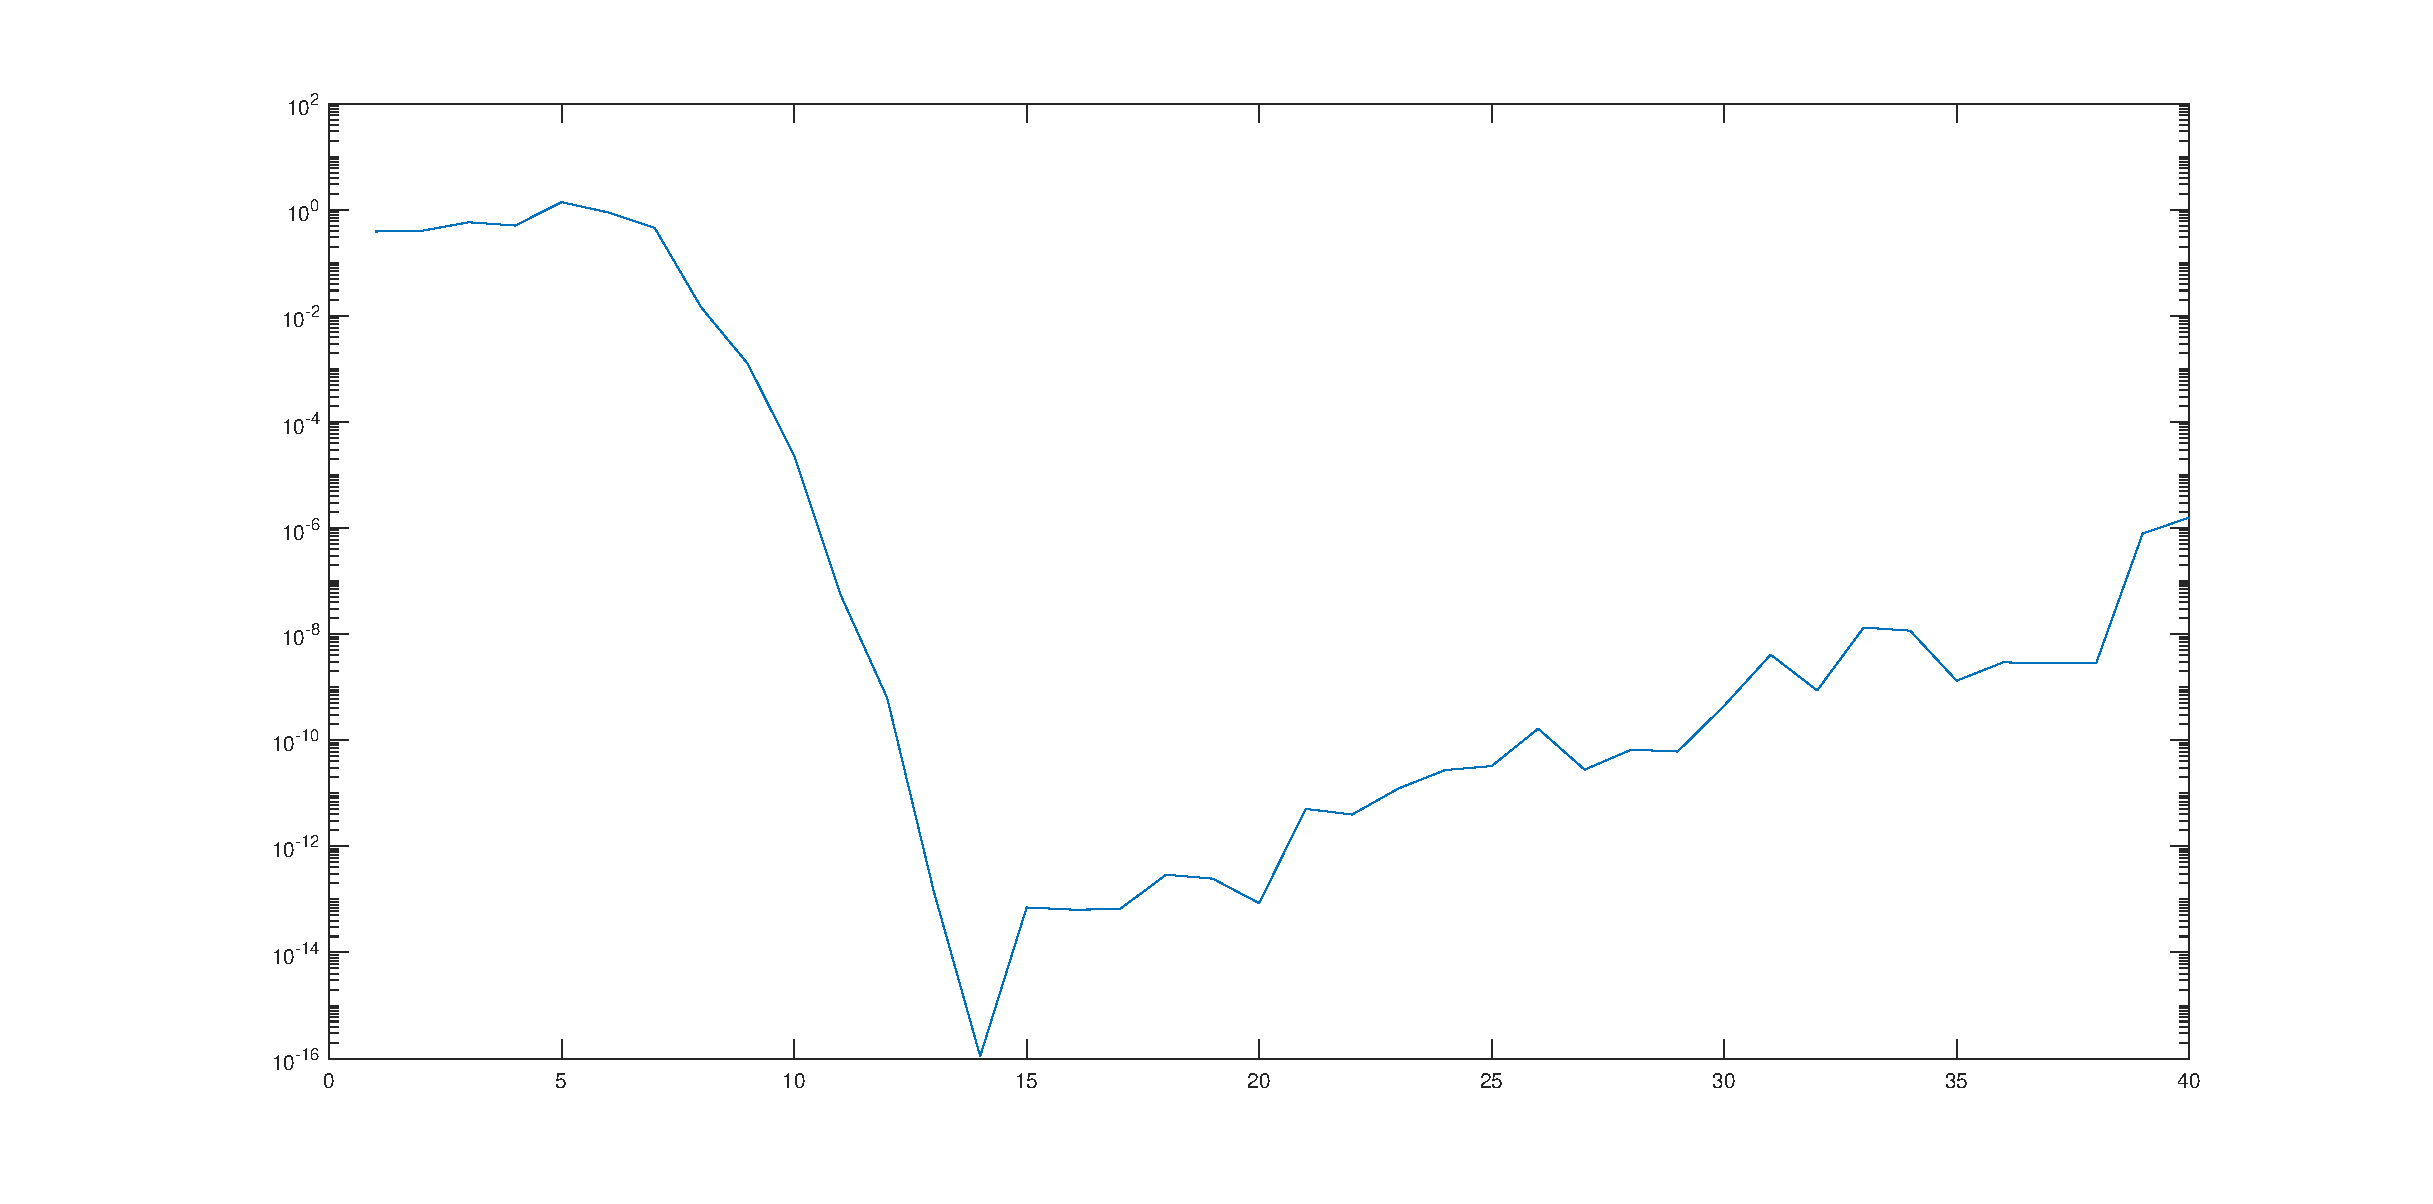
\includegraphics[width=\textwidth]{semilogy1}
			\caption{精度随外推次数的变化}  
			\label{2}  
		\end{figure}
		(a)的\textsc{Matlab}程序显示如下:
		\begin{lstlisting}[breaklines,frame=single]
			H=zeros(1,16);
			y=zeros(1,16);
			exact=cos(1.2);
			err=zeros(1,16);
			for i=0:15
			H(i+1)=10^(-i); %设定步长
			y(i+1)=forward(1.2,H(i+1));
			end
			for i=1:16
			err(i)=abs(y(i)-exact);
			end
			loglog(H,err);
			function y=f(x)
			y=sin(x);
			end
			function y=forward(x,h)
			y=(f(x+h)-f(x))/h;
			end
		\end{lstlisting}		
		(c)的\textsc{Matlab}程序显示如下:
		\begin{lstlisting}[breaklines,frame=single]
			N=40;   %最大迭代次数
			exact=cos(1.2);
			err=zeros(1,N);
			A=zeros(N,N);
			X=zeros(1,N);
			h=67;
			for i=1:N
			A(i,1)=forward(h/2^(i-1));
			end
			for k=2:N
				for i=k:N
				A(i,k)=A(i,k-1)+(A(i,k-1)-A(i-1,k-1))/(2^(k-1)-1);
				end
			end
			
			for i=1:N
			err(i)=abs(A(i,i)-exact);
			X(i)=i;
			end
			semilogy(X,err);
			fprintf('%.16f\n',A(14,14)-exact);
			function y=f(x)
			y=sin(x);
			end
			function y=forward(h)
			y=(f(1.2+h)-f(1.2))/h;
			end
		\end{lstlisting}
		
		\item[第二题] \textbf{本题讨论使用复化梯形公式求周期函数的积分。} 
		\item[(a)](10分)证明当$r$不是$m$的整倍数的情况下,使用$m$个子区间的复化梯形公式可以精确积分
		$$\int_{-\pi}^{\pi} \cos (r x) d x \quad \text { 和 } \quad \int_{-\pi}^{\pi} \sin (r x) d x$$
		注意:这一结论类似于课堂上我们定义的代数精度。同时说明如果$r$为$m$的整倍数时复化梯形公式对于上面两个积分会给出怎样的结果。\\
		证明:\\
		对于$\cos(rx)$,由复化梯形的计算公式得:\\
		$$I_{m}(f)=\frac{2\pi}{m}(\sum_{n=1}^{m-1}\cos(\frac{2nr\pi}{m})+\frac{1}{2}(\cos(0)+\cos(2\pi r)))$$ $$
		\sum_{n=1}^{m-1}\cos(\frac{2nr\pi}{m})=\frac{\sin \left(2 r \pi-\frac{r \pi}{m}\right)}{2 \sin \left(\frac{r \pi}{m}\right)}-\frac{1}{2}$$
		当$r$不是$m$的整数倍的时候,$\sin(\frac{r\pi}{m})\neq 0$\\
		$$\text{原式}=-\frac{\sin \left(\frac{r \pi}{m}\right)}{2 \sin \left(\frac{r \pi}{m}\right)}-\frac{1}{2}+\frac{1}{2}(\cos(0)+\cos(2\pi r))=0$$
		$$\because \int_{-\pi}^{\pi} \cos (r x) d x=I_{m}(f)+E_{m}$$
		$$\therefore E_{m}=0$$此时复化梯形公式可以精确积分。\\
		当$r$是$m$的整数倍的时候,假设$r=km,k\in N_{+}$
		$$\sum_{n=1}^{m-1}\cos(\frac{2nr\pi}{m})=\sum_{n=1}^{m-1}\cos(2k\pi n)=m-1$$ $$
		I_{m}(f)=\frac{2\pi}{m}\times(m-1+1)=2\pi,\qquad E_{m}=2\pi$$此时不能精确积分。\\
		对于$\int_{-\pi}^{\pi} \sin (r x) d x$,当$r$不是$m$的整数倍时结论相同(即可以精确积分)\\
		现考虑$r=km$的情况:
		$$I_{m}(f)=\frac{1}{2}(\sin(0)+\sin(2\pi r))+\frac{2\pi}{m}\sum_{n=1}^{m-1}\sin(2k\pi n)=0$$ $$
		E_{m}(f)=T(f)-I_{m}(f)=0$$
	`	此时仍可以精确积分。		
		
		\item[(b)](10分)由于任意的以$2\pi$为周期的周期函数都可以表示为由正弦与余弦函数的线性组合,所以上一问中所证明的定理实际上告诉我们求解一个周期函数的积分的有效方法正是复化梯形公式。现使用复化梯形公式和不同数量的子区间个数来求$f(x) = e^{\cos(x)}$在$[−\pi, \pi]$的积分,并用这个函数的真实积分值作为参照使用\textbf{semilogy}图画出随着子区间数量$m$变化所得到的积分精度的变化。\\
		\begin{figure}[H]  
			\centering
			\includegraphics[width=\textwidth]{semilogy2}
			\caption{精度随自区间数量$m$的变化}  
			\label{3}  
		\end{figure}
		(b)的\textsc{Matlab}程序显示如下:
		\begin{lstlisting}[breaklines,frame=single]
			exact=7.9549265210128452;%精确解(来自Mathematica)
			N=20; %分割区间
			err=zeros(1,N);
			m=linspace(1,N,N);
			for i=1:N	%复化梯形公式
			h=2*pi/m(i);
			x=linspace(-pi,pi,m(i)+1);
			ans=0.5*f(x(1))+0.5*f(x(m(i)+1));
			for j=2:m(i)
			ans=ans+f(x(j));
			end
			ans=ans*h;
			err(i)=abs(ans-exact);
			end
			
			semilogy(m,err);
			
			function y=f(x)
			y=exp(cos(x));
			end
		\end{lstlisting}
		\item[第三题]
		\item[(a)](10分)推导出如下格式的多步法公式:
		\begin{equation}
			y_{n+1}=y_{n-1}+\alpha f_{n+1}+\beta f_{n}+\gamma f_{n-1}
		\end{equation}
		解:由数值积分公式得\\$$
		\alpha=\int_{x_{n-1}}^{x_{n+1}} \frac{\left(x-x_{n}\right)\left(x-x_{n-1}\right)}{\left(x_{n+1}-x_{n}\right)\left(x_{n+1}-x_{n-1}\right)} dx = \frac{h}{3}$$
		$$\beta=\int_{x_{n-1}}^{x_{n+1}} \frac{\left(x-x_{n+1}\right)\left(x-x_{n-1}\right)}{\left(x_{n+1}-x_{n}\right)\left(x_{n+1}-x_{n-1}\right)} dx = \frac{4h}{3}$$
		$$\gamma=\int_{x_{n-1}}^{x_{n+1}} \frac{\left(x-x_{n+1}\right)\left(x-x_{n}\right)}{\left(x_{n+1}-x_{n}\right)\left(x_{n+1}-x_{n-1}\right)} dx = \frac{h}{3}$$
		因此$$y_{n+1}=y_{n-1}+\frac{h}{3} f_{n+1}+\frac{4h}{3} f_{n}+\frac{h}{3} f_{n-1}$$
		\item[(b)](10分)推导此格式的局部截断误差,并由此指明此格式的阶数。
		假设前$n$步的计算结果都是准确的,则有\\ $$
		y_{n-1}=y(x_{n-1})=y_{n}-y_{n}^{\prime} h+\frac{y_{n}^{\prime \prime}}{2 !} h^{2}-\frac{y_{n}^{\prime \prime \prime}}{3 !} h^{3}+\frac{y_{n}^{(4)}}{4!}h^{4}-\frac{y_{n}^{(5)}}{5 !} h^{5}+O\left(h^{6}\right)$$ $$
		f_{n+1}\approx y^{\prime}\left(x_{n+1}\right)=y_{n}^{\prime}+y_{n}^{\prime \prime} h+\frac{y_{n}^{\prime \prime}}{2 !} h^{2}+\frac{y_{n}^{(4)}}{3 !} h^{3}+\frac{y_{n}^{(5)}}{4 !} h^{4}+O\left(h^{5}\right)$$ $$
		f_{n}=f\left(x_{n}, y_{n}\right)=y^{'}_{n}\qquad (*)$$ $$
		f_{n-1}=y^{\prime}\left(x_{n-1}\right)=y_{n}^{\prime}-y_{n}^{\prime \prime} h+\frac{y_{n}^{\prime \prime \prime}}{2 !} h^{2}-\frac{y_{n}^{(4)}}{3 !} h^{3}+\frac{y_{n}^{(5)}}{4 !} h^{4}+O\left(h^{5}\right)$$
		全部带入(a)中公式得$$
		y_{n+1}=y_{n}+y_{n}^{\prime} h+\frac{y_{n}^{\prime \prime}}{2 !} h^{2}+\cdots+\frac{7y_{n}^{(5)}}{360} h^{5}+O\left(h^{6}\right)$$
		而$$
		y(x_{n+1})=y_{n}+y_{n}^{\prime} h+\frac{y_{n}^{\prime \prime}}{2 !} h^{2}+\cdots+\frac{y_{n}^{(5)}}{5 !} h^{5}+O\left(h^{6}\right)$$ $$ 
		\therefore\qquad T_{n+1}=y(x_{n+1})-y_{n+1}=-\frac{1}{90} h^{5}y_{n}^{(5)}+O\left(h^{6}\right)$$
		因此此公式是四阶的。
		\item[(c)](10分)选取合适的步长值,用此格式在[0, 2]上解如下的初值问题:
		\begin{equation}
			y^{\prime}=x e^{-4 x}-4 y, \quad y(0)=0
		\end{equation}
		使用你刚刚推导出的格式(1),并利用二阶\textbf{Runge-Kutta}方法(即课本公式(7.15))起步。画出解函数。
		\begin{figure}[H]  
			\centering
			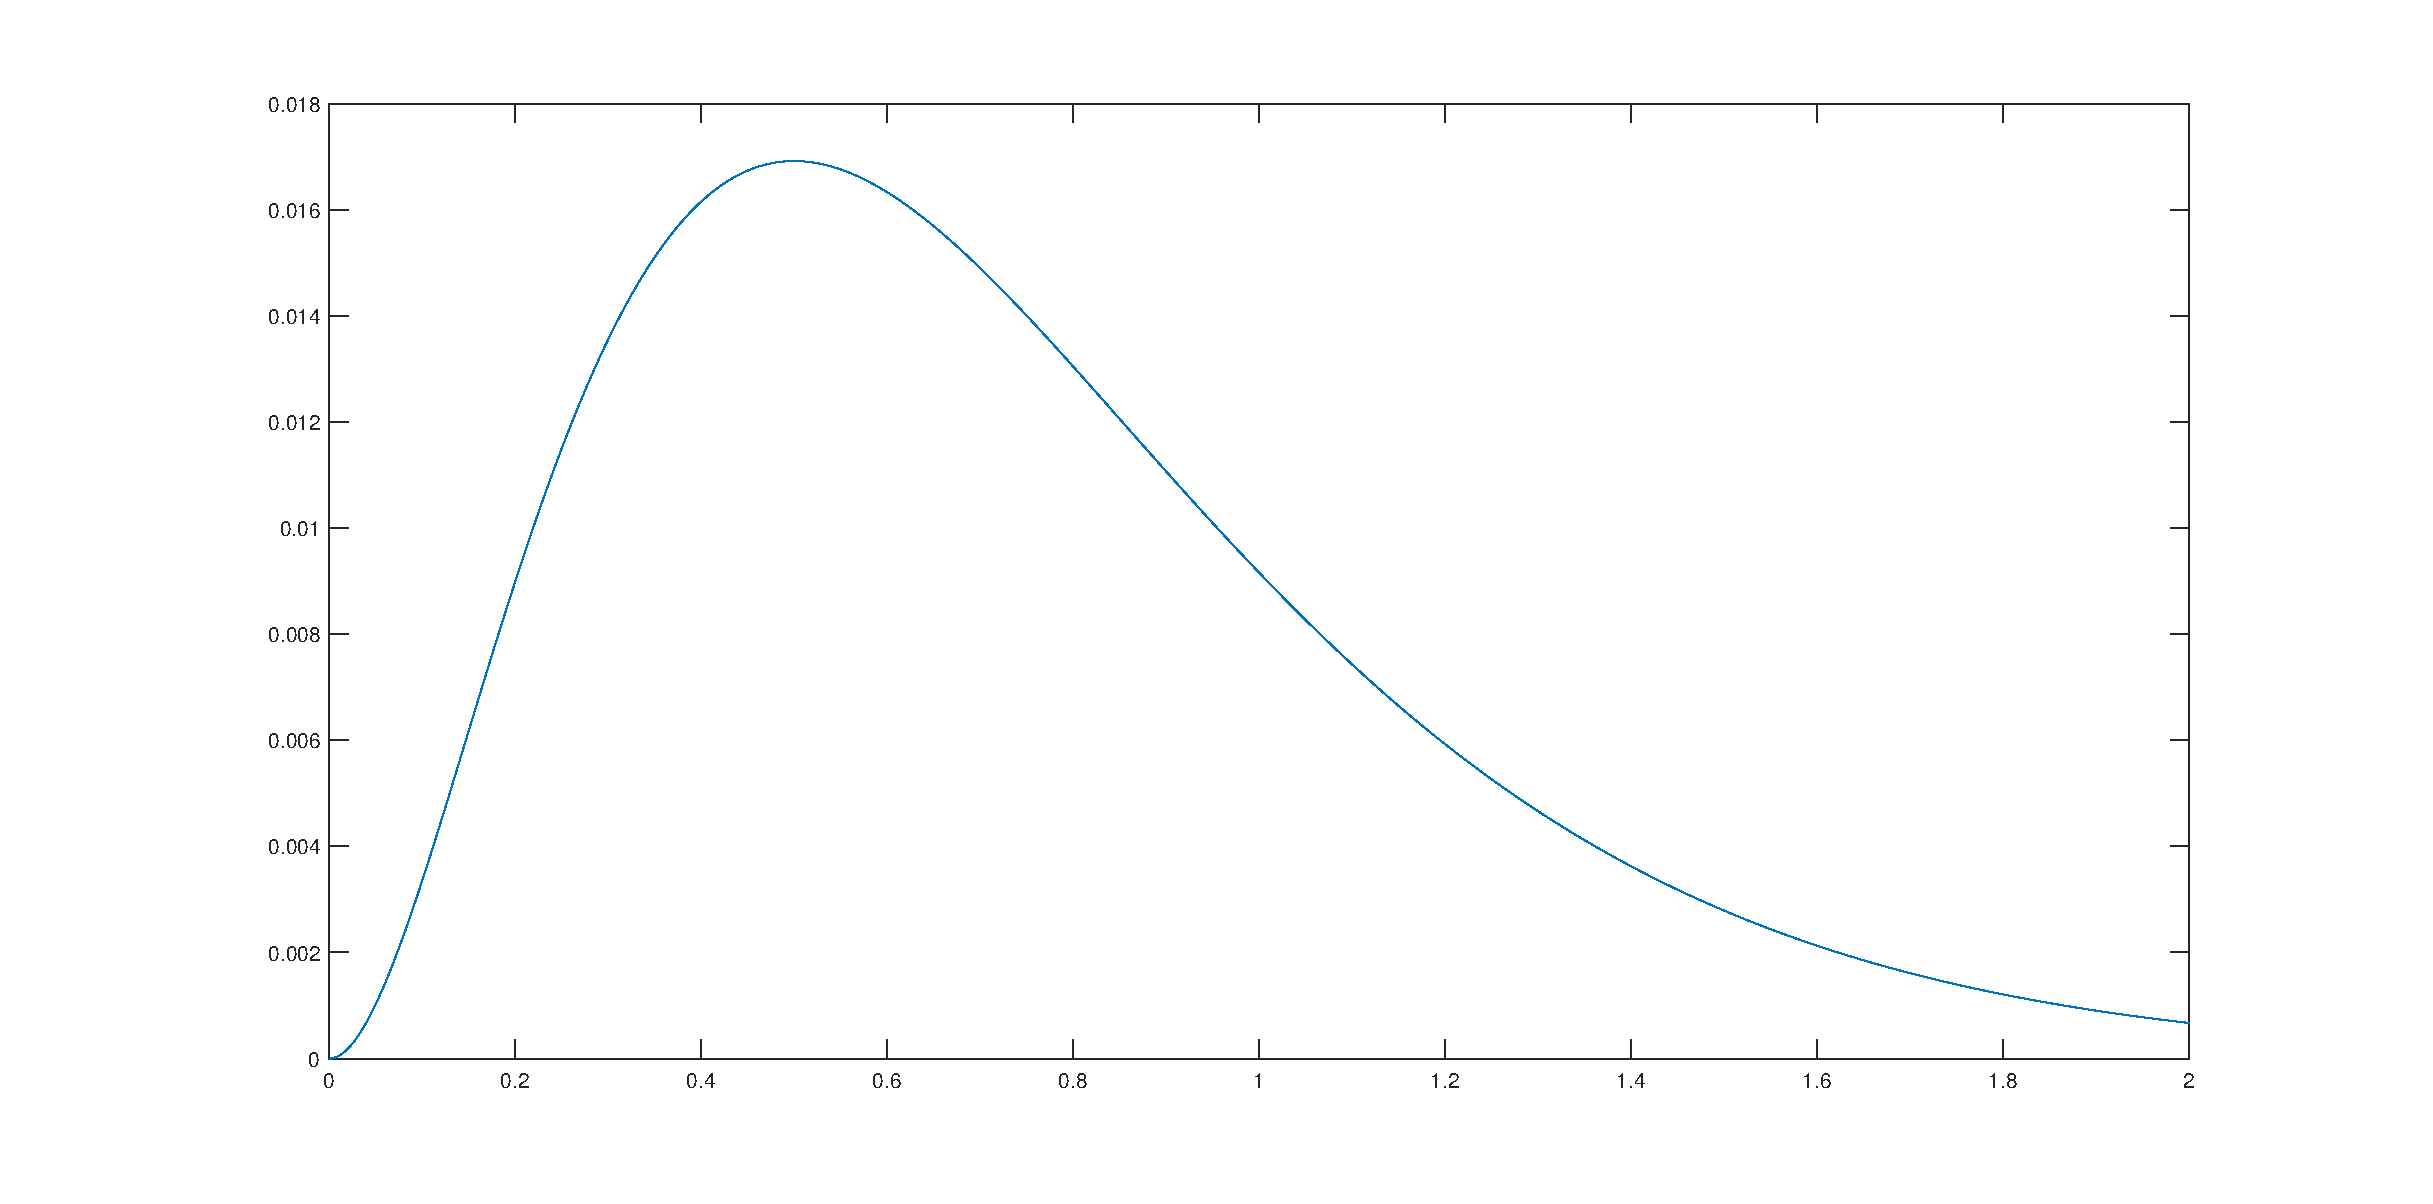
\includegraphics[width=\textwidth]{plot3}
			\caption{解函数的图像}  
			\label{4}  
		\end{figure}
		\item[(d)](10分)推导出(2)的精确解。对比该精确解在$x = 2$这一点的值,用\textbf{log-log}图展示所用方法的阶数,并给出解释。\\
		解:使用常数变易法。\\
		首先计算通解
		$$y^{'}=-4y$$
		解得:$$
		y=C(x)e^{-4x}$$
		代回微分方程得:$$
		C^{'}(x)=x$$ $$
		C(x)=\frac{1}{2}x^{2}+c\quad c\in R$$
		由$y(0)=0$得:\quad$C(x)=\frac{1}{2}x^{2}$ $$\therefore\qquad
		y=\frac{1}{2}x^{2}e^{-4x}$$
		\begin{figure}[H]  
			\centering
			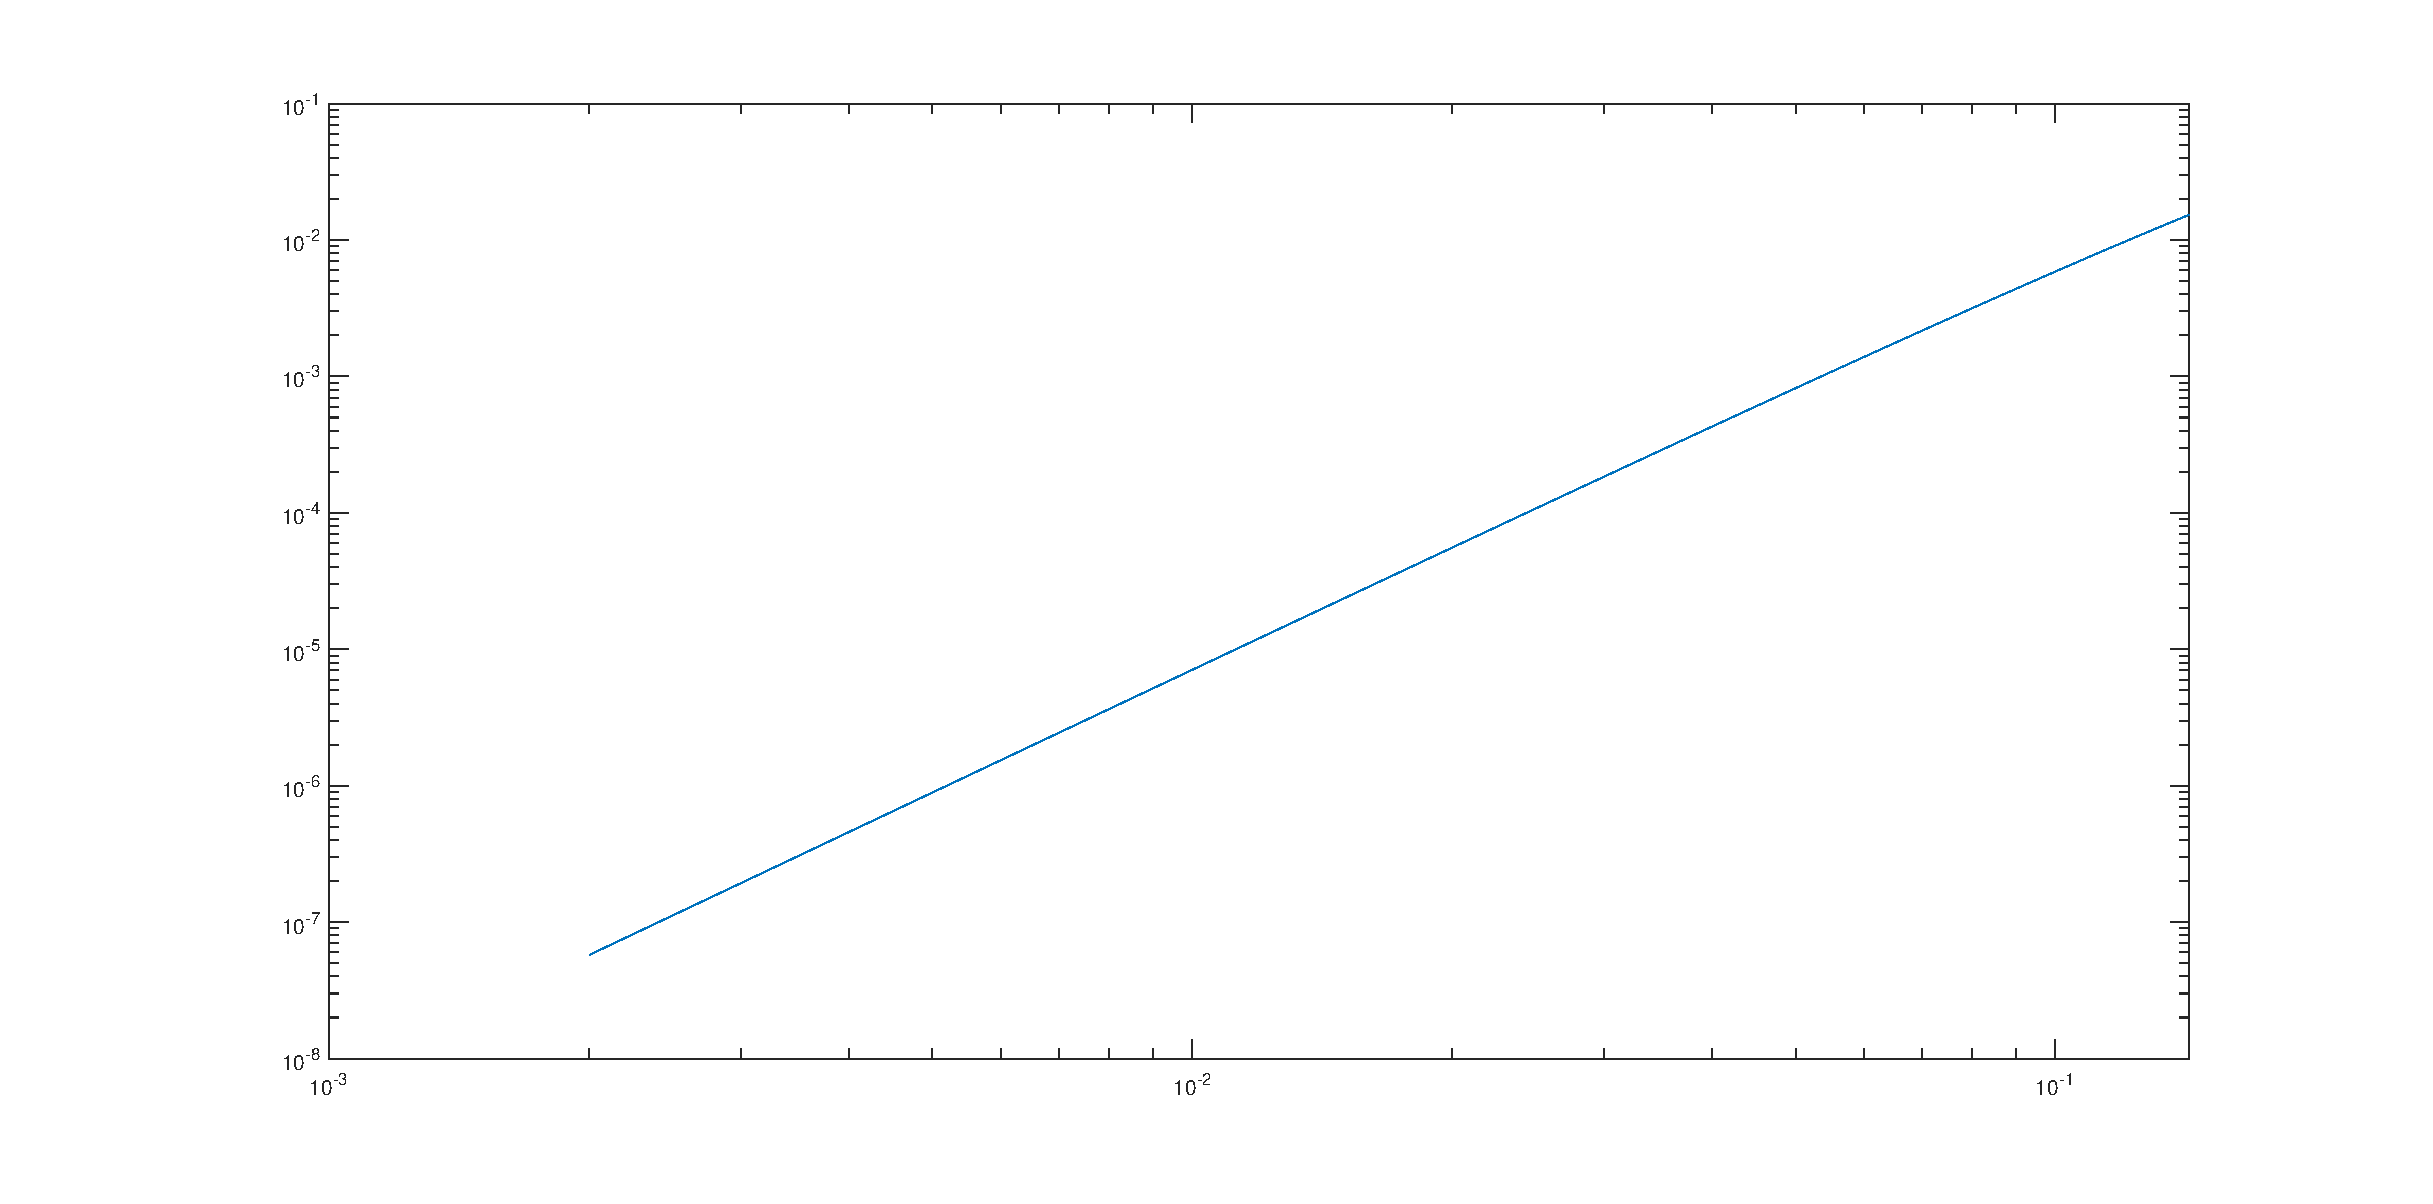
\includegraphics[width=\textwidth]{loglog3}
			\caption{用步长和误差估计阶数}  
			\label{5}  
		\end{figure}
		图像的斜率为3,因此该方法是三阶的\\
		个人分析如下:\\
		由于$y_{1}$是由二阶Runge-Kutta方法得到的,其误差为$O(h^{3})$\\
		因此$y_{1}=y(x_{1}+ch^{3})\qquad c\neq 0$\\
		对于(*),在计算$y_{2}$的时候$y_{1}$扮演$y_{n}$的角色,此时$$
		f_{n}=y^{'}(x_{n}+ch^{3})=y^{'}_{n}+ch^{3}y^{''}_{n}+O(h^{6})$$
		带入$y_{n+1}$的表达式得$$
		y_{n+1}=y_{n}+y_{n}^{\prime} h+\frac{y_{n}^{\prime \prime}}{2 !} h^{2}+\frac{y^{'''}_{n}}{3!}h^{3}+(\frac{4c}{3}y^{''}_{n}+\frac{y^{(4)}_{n}}{4!})h^{
		4}+O(h^{5})$$ $$
		\therefore\qquad T_{n+1}=Ch^{4}+O(h^{5})\qquad C\neq 0$$ 
		因此该方法的阶数为三阶\\
		(c)的\textsc{Matlab}程序显示如下:
		\begin{lstlisting}[breaklines,frame=single]
			N=1000;
			h=2/(N-1);
			x=linspace(0,2,N);
			y=zeros(1,N);
			err=zeros(1,N);
			x(1)=0;y(1)=0;
			k1=f(x(1),y(1));
			k2=f(x(1)+h/2,y(1)+h/2*k1);
			y(2)=y(1)+h*k2;
			err(2)=abs(Y(x(2))-y(2));
			f1=f(x(1),y(1));
			f2=f(x(2),y(2));
			for i=3:N 
			y(i)=3/(3+4*h)*(y(i-2)+h/3*(x(i)*exp(-4*x(i))+4*f2+f1));
			f1=f2;
			f2=f(x(i),y(i));
			end
			plot(x,y)
			
			function s=f(x,y)
			s=x*exp(-4*x)-4*y;
			end
			
			function y=Y(x)
			y=0.5*x^2*exp(-4*x);
			end
		\end{lstlisting}
		(d)的\textsc{Matlab}程序显示如下:
		\begin{lstlisting}[breaklines,frame=single]
			S=15;  %初始区间长度(为了绘图美观从15开始取)
			err=zeros(1,1001-S);
			H=zeros(1,1001-S);
			for N=S:1000
			h=2/(N-1);
			H(N-S+1)=h;
			x=linspace(0,2,N);
			y=zeros(1,N);
			x(1)=0;y(1)=0;
			k1=f(x(1),y(1));
			k2=f(x(1)+h/2,y(1)+h/2*k1);
			y(2)=y(1)+h*k2;
			f1=f(x(1),y(1));
			f2=f(x(2),y(2));
			for i=3:N 
			y(i)=3/(3+4*h)*(y(i-2)+h/3*(x(i)*exp(-4*x(i))+4*f2+f1));
			f1=f2;
			f2=f(x(i),y(i));
			end
			err(N-S+1)=abs(y(N)-Y(2));
			end

			loglog(H,err);
			
			function s=f(x,y)
			s=x*exp(-4*x)-4*y;
			end
			
			function y=Y(x)
			y=0.5*x^2*exp(-4*x);
			end
		\end{lstlisting}
	\end{enumerate}
\end{document}
